\documentclass{jsarticle}
\usepackage[dvipdfmx]{graphicx,color}
\usepackage{ulem}
\usepackage{ascmac}
\usepackage{pgf,tikz}
\usepackage{here}
%\usepackage{subcaption}
\usepackage{amsmath,amssymb}
\usepackage{ascmac}
\usepackage{comment}
\usepackage{theorem}
\newtheorem{theorem}{定理}
\newtheorem{proof}{証明}
\newtheorem{remark}{Remark}
\usepackage{framed}
\def\qed{\hfill $\Box$}
\definecolor{shadecolor}{gray}{0.80}

%\usepackage{showkeys}

\begin{document}
\title{数理解析特論レポート}
\author{米田亮介}
\date{}
\maketitle
\section{Darboux変換}
\begin{shaded}
\begin{enumerate}
\item 差分演算子$L,B$をそれぞれ
$L=e^{\partial/\partial n}+u_{n}e^{-\partial/\partial n},
B=-u_{n}u_{n-1}e^{-2\partial/\partial n}$で定める。
このとき、関数$\varphi_{n}(t)$に対する線形方程式
\begin{align}
L\varphi_{n}(t)=(\lambda+1/\lambda)\varphi_{n}(t),\quad
\frac{d}{dt}\varphi_{n}(t)=B\varphi_{n}(t)
\end{align}
の両立条件から、無限格子上の連続時間発展方程式であるLotka--Voltera(LV)方程式
\begin{align}
\frac{d}{dt}u_{n}=u_{n}(u_{n+1}-u_{n-1})
\end{align}
が導かれることを示せ。
ここで、$\lambda+1/\lambda$は$L$の固有値を与える定数。
\item LV方程式の自明な解$u=1$をseed(種)として、
Darboux変換を$k$回適用することで得られる差分作用素を
$L^{(k)}=e^{\partial/\partial n}+u_{n}^{(k)}e^{-\partial/\partial n}$
で表す。
このとき、$u_{n}^{(1)}$および$u_{n}^{(2)}$を求めよ。
\end{enumerate}
\end{shaded}
関数$f$のシフト演算子$e^{a\partial/\partial x}$は
\begin{align}
e^{a\partial/\partial x}f(x)=f(x+a)
\end{align}
で書けるのであった\footnote{
	直観的にはテイラー展開によって説明できる。
	$C^{\omega}$級の関数$f$について
	\begin{align*}
		e^{a\partial/\partial x}f(x)
		=\sum_{n=0}^{\infty}\frac{a^{n}}{n!}\left(\frac{\partial}{\partial x}\right)^{n}f(x)
		=\sum_{n=0}^{\infty}\frac{a^{n}}{n!}f^{(n)}(x)
		=f(x+a)
	\end{align*}
	と形式的に書ける。
	有限回の微分操作では局所的な作用素にしかなりえないが、
	無限回の微分操作まで含めると、こういった大域的な演算子を生成することが出来るようになる。
	このことは有限と無限の違いを浮き彫りにする一つの面白い結果だと思う。
}。
本レポートでは関数のシフト演算子の類似として数列$u_{n}$に作用するシフト演算子$e^{k\partial/\partial n}$は
\begin{align}
e^{k\partial/\partial n}u_{n}=u_{n+k}
\end{align}
で作用するように決めることにする。
\begin{enumerate}
\item 線形方程式
\begin{align}
L\varphi_{n}(t)=(\lambda+1/\lambda)\varphi_{n}(t)
\end{align}
の両辺を$t$微分すると、
\begin{align}
\begin{split}
L_{t}\varphi_{n}(t)
&=(\lambda+1/\lambda)\frac{d}{dt}\varphi_{n}(t)
-L\frac{d}{dt}\varphi_{n}(t)\\
&=(\lambda+1/\lambda)B\varphi_{n}(t)-LB\varphi_{n}(t)\\
&=B\left[(\lambda+1/\lambda)\varphi_{n}(t)\right]-LB\varphi_{n}(t)\\
&=(BL-LB)\varphi_{n}(t)
\end{split}
\end{align}
が成り立つ必要がある。これより、両立条件
\begin{align}
L_{t}=BL-LB
\end{align}
が必要となる。
\begin{align}
\begin{split}
L_{t}&=\frac{du_{n}}{dt}e^{-\partial/\partial n},
\end{split}\\
\begin{split}
BL-LB&=-u_{n}u_{n-1}e^{-2\partial/\partial n}\left(e^{\partial/\partial n}+u_{n}e^{-\partial n}\right)
+\left(e^{\partial/\partial n}+u_{n}e^{-\partial n}\right)\left(u_{n}u_{n-1}e^{-2\partial/\partial n}\right)\\
&=-u_{n}u_{n-1}e^{-\partial/\partial n}-u_{n}u_{n-1}u_{n-2}e^{-3\partial/\partial n}
+u_{n+1}u_{n}e^{-\partial/\partial n}+u_{n}u_{n-1}u_{n-2}e^{-3\partial/\partial n}\\
&=u_{n}(u_{n+1}-u_{n-1})e^{-\partial/\partial n}
\end{split}
\end{align}
が計算によりわかるので、係数比較により
\begin{align}
\frac{du_{n}}{dt}=u_{n}(u_{n+1}-u_{n-1})
\end{align}
となり、LV方程式が得られた。

\item 
LV方程式におけるDarboux変換を簡単に復習する。
$k$回目のDarboux変換により得られたLV方程式の解を$u^{(k)}_{n}$とおく。
そのときの差分演算子を$L^{(k)}=e^{\partial/\partial n}+u^{(k)}_{n}e^{-\partial/\partial n},
B^{(k)}=-u_{n}^{(k)}u_{n-1}^{(k)}e^{-2\partial/\partial n}$で表すことにする。
この差分演算子で表された差分方程式を満たす固有関数を$\varphi_{n}^{(k)}$と書くことにする。
このとき、
\begin{align}
F^{(k)}L^{(k)}=L^{(k+1)}F^{(k)}
\end{align}
を満足する作用素$L^{(k+1)},F^{(k)}$を見つけることができれば、
$\varphi_{n}^{(k+1)}:=F^{(k)}\varphi_{n}^{(k)}$によって、
\begin{align}
L^{(k+1)}\varphi_{n}^{(k+1)}=L^{(k+1)}F^{(k)}\varphi_{n}^{(k)}
=F^{(k)}L^{(k)}\varphi_{n}^{(k)}=\eta(\lambda)F^{(k)}\varphi_{n}^{(k)}
=\eta(\lambda)\varphi_{n}^{(k+1)}
\end{align}
となり、新たな固有関数$\varphi_{n}^{(k+1)}$を生成することが出来る。
このとき、作用素$F^{(k)}$の一つ(配布レポートの裏側による)として次が得られる。
\begin{align}
\left\{
\begin{array}{l}
F^{(k)}=e^{2\partial/\partial n}-A_{n}^{(k)}\\
A_{n}^{(k)}=\dfrac{\varphi_{n+2}^{(k)}}{\varphi_{n}^{(k)}}
\end{array}
\right.
\end{align}
また、$u_{n}^{(k)}$は次の漸化式によって得られる。
\begin{align}
u_{n}^{(k+1)}=\frac{A_{n}}{A_{n-1}}u_{n}^{(k)}
\end{align}

以上を踏まえて$u^{(0)}_{n}=1$(自明解)として実際にDarboux変換を施していく。
はじめに$\varphi_{n}^{(0)}$を求める。$L^{(0)}\varphi_{n}^{(0)}=\eta(\lambda)\varphi_{n}^{(0)}$より、
\begin{align}
\varphi_{n+1}^{(0)}-(\lambda+1/\lambda)\varphi_{n}^{(0)}+\varphi_{n-1}^{(0)}=0
\end{align}
となる。これを解くと、
\begin{align}
\varphi_{n}^{(0)}=\tilde{c_{1}}\lambda^{n}+\tilde{c_{2}}\lambda^{-n}
\end{align}
となる。次に$\varphi_{n}^{(0)}$の時間発展を考える。$\frac{d\varphi_{n}^{(0)}}{dt}=B^{(0)}\varphi_{n}^{(0)}$より、
\begin{align}
\frac{d\tilde{c_{1}}}{dt}\lambda^{n}+\frac{d\tilde{c_{2}}}{dt}\lambda^{-n}
=-\tilde{c_{1}}\lambda^{n-2}-\tilde{c_{2}}\lambda^{-n+2}
\end{align}
である。これより、
\begin{align}
\frac{d\tilde{c_{1}}}{dt}=-\frac{1}{\lambda^{2}}\tilde{c_{1}},\quad
\frac{d\tilde{c_{2}}}{dt}=-\lambda^{2}\tilde{c_{2}}
\end{align}
であるから、これを解くと、
\begin{align}
\varphi_{n}^{(0)}=c_{1}\lambda^{n}e^{-t/\lambda^{2}}+c_{2}\lambda^{-n}e^{-\lambda^{2}t}
\end{align}
がわかる。ここで$c_{1},c_{2}$は任意定数である。
これより、$u_{n}^{(0)}$のDarboux変換$u_{n}^{(1)}$は、
\begin{align}
u_{n}^{(1)}=\frac{A_{n}}{A_{n-1}}u_{n}^{(0)}
=\frac{\varphi_{n+2}^{(0)}\varphi_{n-1}^{(0)}}{\varphi_{n}^{(0)}\varphi_{n-1}^{(0)}}
=\frac{(c_{1}\lambda^{n+2}e^{-t/\lambda^{2}}+c_{2}\lambda^{-n-2}e^{-\lambda^{2}t})(c_{1}\lambda^{n-1}e^{-t/\lambda^{2}}+c_{2}\lambda^{-n+1}e^{-\lambda^{2}t})}{(c_{1}\lambda^{n}e^{-t/\lambda^{2}}+c_{2}\lambda^{-n}e^{-\lambda^{2}t})(c_{1}\lambda^{n+1}e^{-t/\lambda^{2}}+c_{2}\lambda^{-n-1}e^{-\lambda^{2}t})}
\end{align}
である。$c_{1}$もしくは$c_{2}$を$0$とすると$u_{n}^{(1)}=1$となってしまうので、
どちらも$0$ではない。
これより、$c=c_{2}/c_{1}$とおくことで、
\begin{align}
u_{n}^{(1)}=\frac{(\lambda^{n+2}e^{-t/\lambda^{2}}+c\lambda^{-n-2}e^{-\lambda^{2}t})(\lambda^{n-1}e^{-t/\lambda^{2}}+c\lambda^{-n+1}e^{-\lambda^{2}t})}{(\lambda^{n}e^{-t/\lambda^{2}}+c\lambda^{-n}e^{-\lambda^{2}t})(\lambda^{n+1}e^{-t/\lambda^{2}}+c\lambda^{-n-1}e^{-\lambda^{2}t})}
\end{align}
が得られる。

次に、$u_{n}^{(2)}$を求めるために、$\varphi_{n}^{(1)}$を求める。
$\varphi_{n}^{(1)}$はLax pairを満たすことから、
\begin{align}
\left\{
\begin{array}{l}
\varphi_{n+1}^{(1)}-(\lambda+1/\lambda)\varphi_{n}^{(1)}+u_{n}^{(1)}\varphi_{n-1}^{(1)}=0\\
\dfrac{d\varphi_{n}^{(1)}}{dt}=-u_{n}^{(1)}u_{n-1}^{(1)}\varphi_{n}^{(1)}
\end{array}
\right.
\end{align}
を解く必要がある。が、これ以上解くことが出来なかったため、$u_{n}^{(2)}$を求めることは出来なかった。
\end{enumerate}

\section{離散系・超離散系}
\begin{shaded}
離散Lotka--Voltera(dLV)方程式
\begin{align}
\frac{V_{n}^{(t+1)}}{V_{n}^{(t)}}=\frac{1+\delta V_{n-1}^{(t)}}{1+\delta V_{n+1}^{(t+1)}}
\end{align}
について考える。
\begin{enumerate}
\item 双線形dLV方程式
\begin{align}
(1+\delta)\tau_{n-1}^{(t+1)}\tau_{n}^{(t)}=\tau_{n-1}^{(t)}\tau_{n}^{(t+1)}+\delta\tau_{n-2}^{(t)}\tau_{n+1}^{(t+1)}
\end{align}
に対して、従属変数変換
\begin{align}
V_{n}^{(t)}=\frac{\tau_{n-1}^{(t)}\tau_{n+2}^{(t+1)}}{\tau_{n}^{(t)}\tau_{n+1}^{(t+1)}}
\end{align}
を施すことで、dLV方程式を導出せよ。
\item 双線形dLV方程式が1ソリトン解
\begin{align}
&\tau_{n}^{(t)}=1+\alpha p^{n}q^{t},\\
&q=\frac{1+\delta(1+\delta)^{-1}p^{-1}}{1+\delta(1+\delta)^{-1}p}
\end{align}
を満たすことを確かめよ。
\item dLV方程式から超離散Lotka--Voltera方程式を導出せよ。
\item 双線形dLV方程式の1ソリトン解$\tau_{n}^{(t)}$の超離散化から
超離散Lotka--Voltera方程式の1ソリトン解$T_{n}^{(t)}$を導出せよ。
\item dLV方程式の1ソリトン解に対して次のパラメータ変換を導入する。
\begin{align}
p=\exp(P/\varepsilon),\quad
\delta=\exp(-1/\varepsilon),\quad
\alpha=\exp(A/\varepsilon).
\end{align}
このとき、$\varepsilon=0.1,0.05,0.001$などと$\varepsilon$を選び、
離散Lotka--Voltera方程式の解を用いて$U_{n}^{(t)}=\varepsilon\log V_{n}^{(t)}$を
プロットすることで、超離散系への移行の様子を観察せよ。
\end{enumerate}
\end{shaded}
\begin{enumerate}
\item 双線形dLV方程式を$n\to n+1$にシフトして整理すると、
\begin{align}
\begin{split}
&(1+\delta)\tau_{n}^{(t+1)}\tau_{n+1}^{(t)}=\tau_{n}^{(t)}\tau_{n+1}^{(t+1)}
+\delta\tau_{n-1}^{(t)}\tau_{n+2}^{(t+1)}
\\
\Leftrightarrow&
V_{n}^{(t)}=\frac{\tau_{n-1}^{(t)}\tau_{n+2}^{(t+1)}}{\tau_{n}^{(t)}\tau_{n+1}^{(t+1)}}
=\frac{1+\delta}{\delta}\frac{\tau_{n}^{(t+1)}\tau_{n+1}^{(t)}}{\tau_{n}^{(t)}\tau_{n+1}^{(t+1)}}-\frac{1}{\delta}\\
\Leftrightarrow&
1+\delta V_{n}^{(t)}=(1+\delta)\frac{\tau_{n}^{(t+1)}\tau_{n+1}^{(t)}}
{\tau_{n}^{(t)}\tau_{n+1}^{(t+1)}}
\end{split}
\end{align}
となるから、
\begin{align}
\begin{split}
\frac{1+\delta V_{n-1}^{(t)}}{1+\delta V_{n+1}^{(t+1)}}
&=\frac{\tau_{n-1}^{(t+1)}\tau_{n}^{(t)}}{\tau_{n-1}^{(t)}\tau_{n}^{(t+1)}}
\frac{\tau_{n+1}^{(t+1)}\tau_{n+2}^{(t+2)}}{\tau_{n+1}^{(t+2)}\tau_{n+2}^{(t+1)}}
=\frac{\tau_{n-1}^{(t+1)}\tau_{n+2}^{(t+2)}}{\tau_{n}^{(t+1)}\tau_{n+1}^{(t+2)}}
\frac{\tau_{n}^{(t)}\tau_{n+1}^{(t+1)}}{\tau_{n-1}^{(t)}\tau_{n+2}^{(t+1)}}
=\frac{V_{n}^{(t+1)}}{V_{n}^{(t)}}
\end{split}
\end{align}
となり、dLV方程式が得られた。
\item 
双線形dLV方程式の左辺、右辺それぞれに1ソリトン解$\tau_{n}^{(t)}$を代入すると、
\begin{align}
\begin{split}
(1+\delta)\tau_{n-1}^{(t+1)}\tau_{n}^{(t)}
&=(1+\delta)(1+\alpha p^{n-1}q^{t+1})(1+\alpha p^{n}q^{t})\\
&=(1+\delta)\left[1+\alpha p^{n-1}q^{t}(q+p)+\alpha^{2}p^{2n-1}q^{2t+1}\right],
\end{split}\\
\begin{split}
\tau_{n-1}^{(t)}\tau_{n}^{(t+1)}+\delta\tau_{n-2}^{(t)}\tau_{n+1}^{(t+1)}
&=(1+\alpha p^{n-1}q^{t})(1+\alpha p^{n}q^{t+1})
+\delta(1+\alpha p^{n-2}q^{t})(1+\alpha p^{n+1}q^{t+1})\\
&=1+\alpha p^{n-1}q^{t}(1+pq)+\alpha^{2}p^{2n-1}q^{2t+1}\\
&\qquad+\delta\left[1+\alpha p^{n-2}q^{t}(1+p^{3}q)+\alpha^{2}p^{2n-1}q^{2t+1}\right]
\end{split}
\end{align}
である。左辺から右辺を引くと、
\begin{align}
\begin{split}
&\alpha p^{n-2}q^{t}\left[(1+\delta)p(p+q)-p(1+pq)-\delta(1+p^{3}q)\right]\\
=&\alpha p^{n-2}q^{t}(1-p)\left[p(q-1)+\delta(pq-1)(1+p)\right]\\
=&\alpha p^{n-2}q^{t}(1-p)\left[p\frac{1+\delta+\delta p^{-1}-(1+\delta+\delta p)}{1+\delta+\delta p}-\delta\frac{p(1+\delta+\delta p^{-1})-(1+\delta+\delta p)}{1+\delta+\delta p}(1+p)\right]\\
=&\alpha p^{n-2}q^{t}(1-p)\left[\frac{\delta(1-p)(1+p)}{1+\delta+\delta p}-\frac{\delta(1-p)(1+p)}{1+\delta+\delta p}\right]=0
\end{split}
\end{align}
となる。
以上より、$\tau_{n}^{(t)}$が双線形dLV方程式の解であることが確かめられた。
\item 
dLV方程式
\begin{align}
\frac{V_{n}^{(t+1)}}{V_{n}^{(t)}}=\frac{1+\delta V_{n-1}^{(t)}}{1+\delta V_{n+1}^{(t+1)}}
\end{align}
に対する超離散化を考える。$V_{n}^{(t)},\delta$が正であるとして次の変数変換を施す。
\begin{align}
V_{n}^{(t)}=\exp\left(\frac{W_{n}^{(t)}}{\varepsilon}\right),\quad
\delta=\exp\left(\frac{-L}{\varepsilon}\right).
\end{align}
これをdLV方程式に代入して両辺に$\varepsilon\log$を取ると、
\begin{align}
W_{n}^{(t+1)}-W_{n}^{(t)}=\varepsilon\log\left[1+\exp\left(\frac{W_{n-1}^{(t)}-L}{\varepsilon}\right)\right]
-\varepsilon\log\left[1+\exp\left(\frac{W_{n+1}^{(t+1)}-L}{\varepsilon}\right)\right]
\end{align}
である。$\varepsilon\to+0$の極限操作を行うと、
\begin{align}
W_{n}^{(t+1)}-W_{n}^{(t)}
=\max\{0,W_{n-1}^{(t)}-L\}-\max\{0,W_{n+1}^{(t+1)}-L\}
\end{align}
である\footnote{
ここで用いたのは
\begin{align*}
\lim_{\varepsilon\to+0}\varepsilon\log\left(\exp\left(\frac{A}{\varepsilon}\right)+\exp\left(\frac{B}{\varepsilon}\right)\right)
=\max\{A,B\}
\end{align*}
という非常に簡単な公式である。
}。
これが求める超離散Lotka--Voltera方程式である。
\item 
1ソリトン解$\tau_{n}^{(t)}$の超離散化を考える。
下の問題に倣って次の変数変換を施す。
\begin{align}
\tau_{n}^{(t)}=\exp\left(T_{n}^{(t)}/\varepsilon\right),\quad
p=\exp\left(P/\varepsilon\right),\quad
\delta=\exp\left(-1/\varepsilon\right),\quad
\alpha=\exp\left(A/\varepsilon\right).
\end{align}
1ソリトン解に代入して両辺に$\varepsilon\log$をとると、
\begin{align}
T_{n}^{(t)}=\varepsilon\log\left[
1+\exp\left(\frac{A+nP}{\varepsilon}\right)
\left(
\frac{1+\exp\left(\frac{-1}{\varepsilon}\right)+\exp\left(\frac{-1-P}{\varepsilon}\right)}
{1+\exp\left(\frac{-1}{\varepsilon}\right)+\exp\left(\frac{-1+P}{\varepsilon}\right)}
\right)^{t}
\right]
\label{eq:ud-1soliton}
\end{align}
ここで、$t$乗されている部分に注目すると、十分小さな$\varepsilon>0$について、
\begin{align}
\frac{1+\exp\left(\frac{-1}{\varepsilon}\right)+\exp\left(\frac{-1-P}{\varepsilon}\right)}
{1+\exp\left(\frac{-1}{\varepsilon}\right)+\exp\left(\frac{-1+P}{\varepsilon}\right)}
\approx\exp\left(\frac{R}{\varepsilon}\right)
\end{align}
として、$R$がどうなるかを考える。両辺に$\varepsilon\log$をとると、
\begin{align}
\begin{split}
R&\approx\varepsilon\log\left\{\left[1+\exp\left(\frac{-1}{\varepsilon}\right)+\exp\left(\frac{-1-P}{\varepsilon}\right)\right]-\left[1+\exp\left(\frac{-1}{\varepsilon}\right)+\exp\left(\frac{-1+P}{\varepsilon}\right)\right]\right\}\\
&\approx\max\{0,-1-P\}-\max\{0,-1+P\}
\end{split}
\end{align}
となる。これより、$\varepsilon\to+0$の極限で、
\begin{align}
\begin{split}
T_{n}^{(t)}=\max\left\{0,A+nP+t\max\{0,-1-P\}-t\max\{0,-1+P\}\right\}
\end{split}
\end{align}
となることがわかる。
\item 
dLV方程式の1ソリトン解$V_{n}^{(t)}$は双線形dLV方程式の1ソリトン解$\tau_{n}^{(t)}$を用いて
\begin{align}
V_{n}^{(t)}=\frac{\tau_{n-1}^{(t)}\tau_{n+2}^{(t+1)}}{\tau_{n}^{(t)}\tau_{n+1}^{(t+1)}}
\end{align}
と書けた。
すると、$V_{n}^{(t)}$の超離散化$U_{n}^{(t)}$は
\begin{align}
\begin{split}
U_{n}^{(t)}=&\lim_{\varepsilon\to+0}\varepsilon\log V_{n}^{(t)}
=\lim_{\varepsilon\to+0}\varepsilon\left(\log\tau_{n-1}^{(t)}+\log\tau_{n+2}^{(t+1)}-\log\tau_{n}^{(t)}-\log\tau_{n+1}^{(t+1)}\right)\\
=&T_{n-1}^{(t)}+T_{n+2}^{(t+1)}-T_{n}^{(t)}-T_{n+1}^{(t+1)}
\end{split}
\end{align}
で与えられる。
このときに、パラメータ変換
\begin{align}
p=\exp\left(P/\varepsilon\right),\quad
\delta=\exp\left(-1/\varepsilon\right),\quad
\alpha=\exp\left(A/\varepsilon\right).
\end{align}
を導入した$V_{n}^{(t)}$に対して、$\varepsilon\log V_{n}^{(t)}$と$U_{n}^{(t)}$
を比較することで超離散系への移行の様子を観察する。
今回は$A=1,P=2$の場合について数値計算を行った。他のパラメーターでもソリトンの向きは変わるが、
構造自体は変わらない(同じような形のグラフが得られる。)ので、
他のパラメータについてはここでは結果を載せることはしない。
また、本来$n,t$は整数だが、$U,V$の定義から自然に実数に拡張出来るので、
プロットの際には整数以外のところもプロットした。
そうしたほうが離散解から超離散解への移行が確認しやすいからである。
超離散解$U(n,t)$と離散解の超離散系への移行を表す$\varepsilon\log V(n,t)$をプロットしたものを図~\ref{fig:ud_a1p2}に示す。
$\varepsilon$の値を$0$に近づけるにつれて離散解のグラフが超離散解のグラフに近づいて行くことが
確認できる。

\begin{figure}[H]
\begin{center}
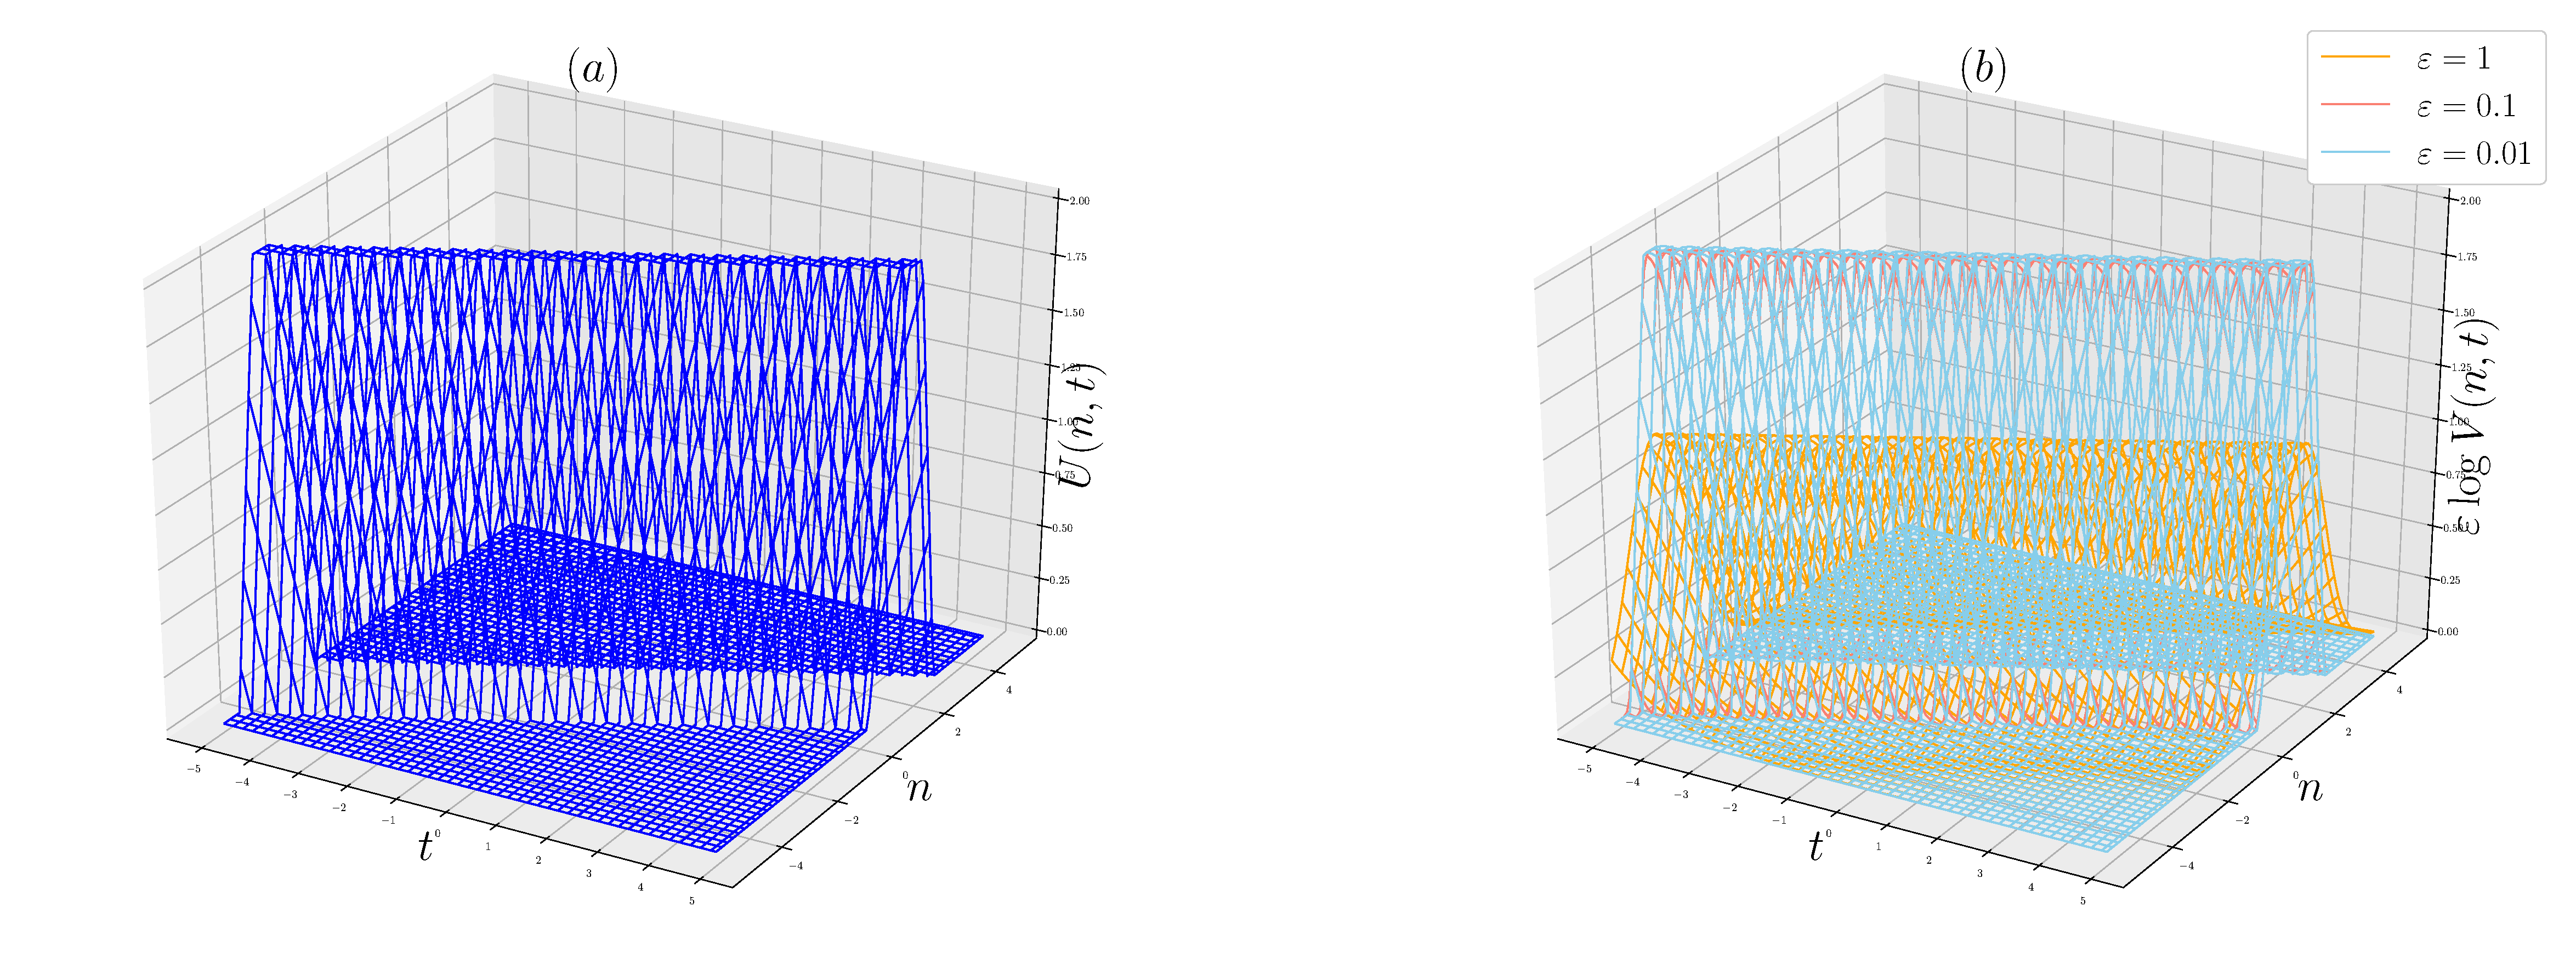
\includegraphics[width=16cm]{lv_a1p3.eps}
\caption{$A=1,P=2$のときの$(a)$超離散解$U(n,t)$と$(b)$離散解$V(n,t)$の超離散系への移行を表す$\varepsilon\log V(n,t)$をプロットしたもの。
$\varepsilon$を小さくするにつれて離散解が超離散解に近づいていることが確認できる。}
\label{fig:ud_a1p2}
\end{center}
\end{figure}

ただ、3次元のグラフだけでは見づらいので、
特に$n=0$において離散解が超離散解に近づいている様子を図~\ref{fig:ud_a1p2_n0}にプロットした。

\begin{figure}[H]
\begin{center}
\includegraphics[width=14cm]{lv_a1p2_n0.eps}
\caption{$n=0$でスライスした、$A=1,P=2$のときの超離散解$U(n,t)$と離散解$V(n,t)$の超離散系への移行を表す$\varepsilon\log V(n,t)$をプロットしたもの。
$\varepsilon$を小さくするにつれて離散解が超離散解に近づいていることが確認できる。}
\label{fig:ud_a1p2_n0}
\end{center}
\end{figure}

以上のように離散解が超離散解に収束していることが確認出来た。
\end{enumerate}
\end{document}